\documentclass[a4paper]{article}

\usepackage[14pt]{extsizes}
\usepackage[T2A]{fontenc}
\usepackage[russian]{babel}

\usepackage[left=20mm, top=15mm, right=15mm, bottom=20mm]{geometry}
\usepackage{listings}
\usepackage{xcolor}
\usepackage{tikz}
\usetikzlibrary{shapes.geometric, arrows.meta, positioning, calc, arrows, shapes.misc}
\usepackage{graphicx}
\usepackage{amsmath}
\usepackage{amssymb}
\usepackage{xcolor}


% -----------------------------------------------------

\newcommand{\labtitle}[7]{
	\begin{center}
		\vspace*{-1.8cm}
		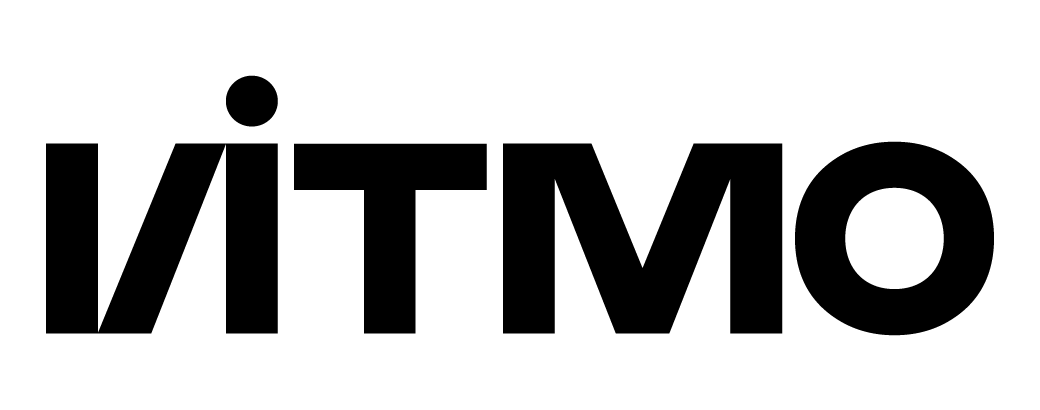
\includegraphics[width=0.26\textwidth]{../common/itmo-logo.png}\\
		\vspace{2.4cm}
		\textbf{\Large Функциональное программирование}\\[1.2cm]
		\textbf{\Large Отчёт по лабораторной работе №#1}\\[0.7cm]
		\textbf{\Large #2}\\[3cm]

		\textbf{\Large Группа \textcolor{red}{\textit{P#3}}}\\[0.2cm]
		\textbf{\Large Вариант \textcolor{red}{\textit{#4}}}\\[3cm]

		\begin{flushleft}
			\textbf{\large Выполнил: \textcolor{red}{\textit{#5}}}\\[0.5cm]
			\textbf{\large Дата защиты: \textcolor{red}{#6}}\\[0.5cm]
			\textbf{\large Количество баллов: \uline{#7}}\\[2cm]
		\end{flushleft}
	\end{center}

	\vspace*{\fill}
	\begin{center}
		\textbf{\Large СПб -- 2024}
	\end{center}
	\vspace*{-1.8cm}
}

% listing for programming code blocks
\definecolor{commentgreen}{RGB}{2,112,10}
\definecolor{eminence}{RGB}{108,48,130}
\definecolor{weborange}{RGB}{255,165,0}
\definecolor{frenchplum}{RGB}{129,20,83}


\lstdefinelanguage{elixir}{
	morekeywords={case,catch,def,do,else,false,%
			use,alias,receive,timeout,defmacro,defp,%
			for,if,import,defmodule,defprotocol,%
			nil,defmacrop,defoverridable,defimpl,%
			super,fn,raise,true,try,end,with,%
			unless},
	otherkeywords={<-,->, |>, \%\{, \}, \{, \, (, )},
	sensitive=true,
	morecomment=[l]{\#},
	morecomment=[n]{/*}{*/},
	morecomment=[s][\color{purple}]{:}{\ },
	morestring=[s][\color{orange}]"",
	commentstyle=\color{commentgreen},
	keywordstyle=\color{eminence},
	stringstyle=\color{red},
	basicstyle=\ttfamily,
	breaklines,
	showstringspaces=false,
	frame=tb
}

\lstset{numbers=left,xleftmargin=2em,frame=single,framexleftmargin=0em,numberstyle=\footnotesize\ttfamily}

% \input{../common/tikzset.tex}

\begin{document}

% Title page

% laboratory work title
\labtitle{1}{Решение задач проекта Эйлер на Elixir}{3331}{9,21}{Дворкин Борис Александрович}{05.10.2024}{}
\thispagestyle{empty}

% -------------------------------

% Main content
\newpage
\thispagestyle{empty}

% Enable text numbering
% \pagestyle{plain}
% \setcounter{page}{1}

\section*{Задача 9}

\textbf{Условие:}

Существуют такие натуральные числа $a$, $b$ и $c$, что:
\[
	a^2 + b^2 = c^2, \text{при } a + b + c = 1000
\]
Нужно найти произведение этих чисел $abc$.

\subsection*{Ключевые элементы реализации}

\subsubsection*{Решение с использованием потоков (Stream):}

\begin{lstlisting}[language=elixir, caption={Генерация чисел с использованием Stream},captionpos=b]
defmodule Euler9Stream do
  def find_triplet(sum) do
    Stream.iterate(1, &(&1 + 1))
    |> Stream.take_while(&(&1 < sum / 3))
    |> Stream.flat_map(fn a ->
      Stream.iterate(a + 1, &(&1 + 1))
      |> Stream.take_while(&(&1 < sum / 2))
      |> Stream.map(fn b ->
        c = sum - a - b
        {a, b, c}
      end)
    end)
    |> Stream.filter(fn {a, b, c} -> a * a + b * b == c * c end)
    |> Enum.map(fn {a, b, c} -> a * b * c end)
    |> Enum.at(0)
  end
end
\end{lstlisting}

\textit{Этот код использует потоки для генерации чисел $a$, $b$, $c$ и фильтрации только тех, которые удовлетворяют условию Пифагора.}

\subsubsection*{Решение с использованием модульного подхода:}

\begin{lstlisting}[language=elixir, caption={Генерация чисел с использованием диапазонов},captionpos=b]
defmodule Euler9Modular do
  def find_triplet(sum) do
    1..(sum - 2)
    |> Enum.flat_map(fn a ->
      (a + 1)..(sum - a - 1)
      |> Enum.map(fn b ->
        c = sum - a - b
        {a, b, c}
      end)
    end)
    |> Enum.filter(fn {a, b, c} -> a * a + b * b == c * c end)
    |> Enum.map(fn {a, b, c} -> a * b * c end)
    |> Enum.at(0)
  end
end
\end{lstlisting}

\textit{Модульный подход использует диапазоны для генерации возможных значений $a$, $b$, $c$.}

\section*{Задача 21}

\textbf{Условие:}

Определим $d(n)$ как сумму всех собственных делителей числа $n$ (чисел меньше $n$, на которые $n$ делится нацело). Если $d(a) = b$ и $d(b) = a$, где $a \neq b$, то $a$ и $b$ — дружественная пара, а $a$ и $b$ называются дружественными числами.

Например, собственные делители $220$ — $1, 2, 4, 5, 10, 11, 20, 22, 44, 55$ и $110$, поэтому $d(220) = 284$. Собственные делители $284$ — $1, 2, 4, 71$ и $142$, так что $d(284) = 220$.

Необходимо найти сумму всех дружественных чисел меньше $10000$.

\subsection*{Ключевые элементы реализации}

\subsubsection*{Решение с использованием потоков (Stream):}

\begin{lstlisting}[language=elixir, caption={Использование потоков для нахождения дружественных чисел},captionpos=b]
defmodule Euler21Stream do
  def sum_amicable_numbers(limit) do
    Stream.iterate(2, &(&1 + 1))
    |> Stream.take_while(&(&1 < limit))
    |> Stream.filter(&amicable?/1)
    |> Enum.sum()
  end

  defp amicable?(n) do
    sum_div = sum_of_divisors(n)
    sum_div != n and sum_div < limit() and sum_of_divisors(sum_div) == n
  end

  defp sum_of_divisors(n) do
    if n > 1 do
      1..div(n, 2)
      |> Enum.filter(&(rem(n, &1) == 0))
      |> Enum.sum()
    else
      0
    end
  end

  defp limit, do: 10_000
end
\end{lstlisting}

\textit{Использование потоков позволяет эффективно фильтровать дружественные числа.}

\subsubsection*{Модульное решение:}

\begin{lstlisting}[language=elixir, caption={Модульный подход к поиску дружественных чисел},captionpos=b]
defmodule Euler21Modular do
  def sum_amicable_numbers(limit) do
    2..(limit - 1)
    |> Enum.filter(&amicable?/1)
    |> Enum.sum()
  end

  defp amicable?(n) do
    sum_div = sum_of_divisors(n)
    sum_div != n and sum_div < limit() and sum_of_divisors(sum_div) == n
  end

  defp sum_of_divisors(n) do
    if n > 1 do
      1..div(n, 2)
      |> Enum.filter(&(rem(n, &1) == 0))
      |> Enum.sum()
    else
      0
    end
  end

  defp limit, do: 10_000
end
\end{lstlisting}

\textit{Модульный подход использует диапазоны и фильтрацию для нахождения дружественных чисел.}

\subsubsection*{Рекурсивное решение:}

\begin{lstlisting}[language=elixir, caption={Рекурсивный подход к поиску дружественных чисел},captionpos=b]
defmodule Euler21Recursion do
  def sum_amicable_numbers(limit) do
    do_sum(2, limit, [])
  end

  defp do_sum(n, limit, acc) when n < limit do
    sum_div = sum_of_divisors(n)

    if sum_div != n and sum_of_divisors(sum_div) == n do
      do_sum(n + 1, limit, [n | acc])
    else
      do_sum(n + 1, limit, acc)
    end
  end

  defp do_sum(_, _, acc), do: Enum.sum(acc)

  defp sum_of_divisors(n), do: sum_of_divisors(n, div(n, 2), 0)

  defp sum_of_divisors(_, i, acc) when i <= 0, do: acc

  defp sum_of_divisors(n, i, acc) do
    if rem(n, i) == 0 do
      sum_of_divisors(n, i - 1, acc + i)
    else
      sum_of_divisors(n, i - 1, acc)
    end
  end
end
\end{lstlisting}

\textit{Использование рекурсии для нахождения суммы дружественных чисел.}

\subsubsection*{Решение на основе Map:}

\begin{lstlisting}[language=elixir, caption={Использование Map для нахождения дружественных чисел},captionpos=b]
defmodule Euler21Map do
  def sum_amicable_numbers(limit) do
    2..(limit - 1)
    |> Enum.map(&{&1, sum_of_divisors(&1)})
    |> Enum.filter(fn {n, sum_div} ->
      sum_div != n and sum_div < limit and sum_of_divisors(sum_div) == n
    end)
    |> Enum.map(fn {n, _} -> n end)
    |> Enum.sum()
  end

  defp sum_of_divisors(n) do
    if n > 1 do
      1..div(n, 2)
      |> Enum.filter(&(rem(n, &1) == 0))
      |> Enum.sum()
    else
      0
    end
  end
end
\end{lstlisting}

\textit{Использование функций отображения (Map) для нахождения дружественных чисел.}

\subsubsection*{Решение с использованием списков (List Comprehensions):}

\begin{lstlisting}[language=elixir, caption={Использование списковых выражений для нахождения дружественных чисел},captionpos=b]
defmodule Euler21ListComp do
  def sum_amicable_numbers(limit) do
    for(
      n <- 2..(limit - 1),
      amicable?(n),
      do: n
    )
    |> Enum.sum()
  end

  defp amicable?(n) do
    sum_div = sum_of_divisors(n)
    sum_div != n and sum_div < limit() and sum_of_divisors(sum_div) == n
  end

  defp sum_of_divisors(n) do
    if n > 1 do
      for(
        i <- 1..div(n, 2),
        rem(n, i) == 0,
        do: i
      )
      |> Enum.sum()
    else
      0
    end
  end

  defp limit, do: 10_000
end
\end{lstlisting}

\textit{Использование списковых выражений для поиска дружественных чисел.}

\section*{Выводы}

В ходе решения задач были применены различные техники: потоки, рекурсия, модульный подход, отображения и списковые выражения. Каждая из них предоставляет свои преимущества в определённых условиях. Потоки и рекурсия обеспечивают элегантные решения для большого количества данных, в то время как отображения и списковые выражения упрощают код и делают его более читаемым.

\end{document}
